%\begin{document}
% first step: page classification
\begin{frame}
\frametitle{Page Classification}
The first step:
\begin{itemize}
\item Separate the pages containing at least one image from those
containing none
\item Could serve as pre-processing step in annotating
\item Proof of concept
\end{itemize}
\end{frame}


% Briefly explain HOG features

\subsection{Method}

\begin{frame}
\frametitle{Features}
Local features to capture the difference between text and images:
	\begin{block}{Histogram of Oriented Gradients (HOG)}
		HOG features contain the amount of gradients in a certain image patch.
	\end{block}
	\begin{block}{Steps for computing HOG Features\cite{dalal2005histograms}}
	\begin{enumerate}
		\item Global image normalisation
		\item Compute the gradient images
		\item Compute gradient histograms in 8 directions
		\item Normalise across blocks
		\item Flatten into a feature vector
	\end{enumerate}
	\end{block}
\end{frame}

\begin{frame}[allowframebreaks]{HOG Examples}
	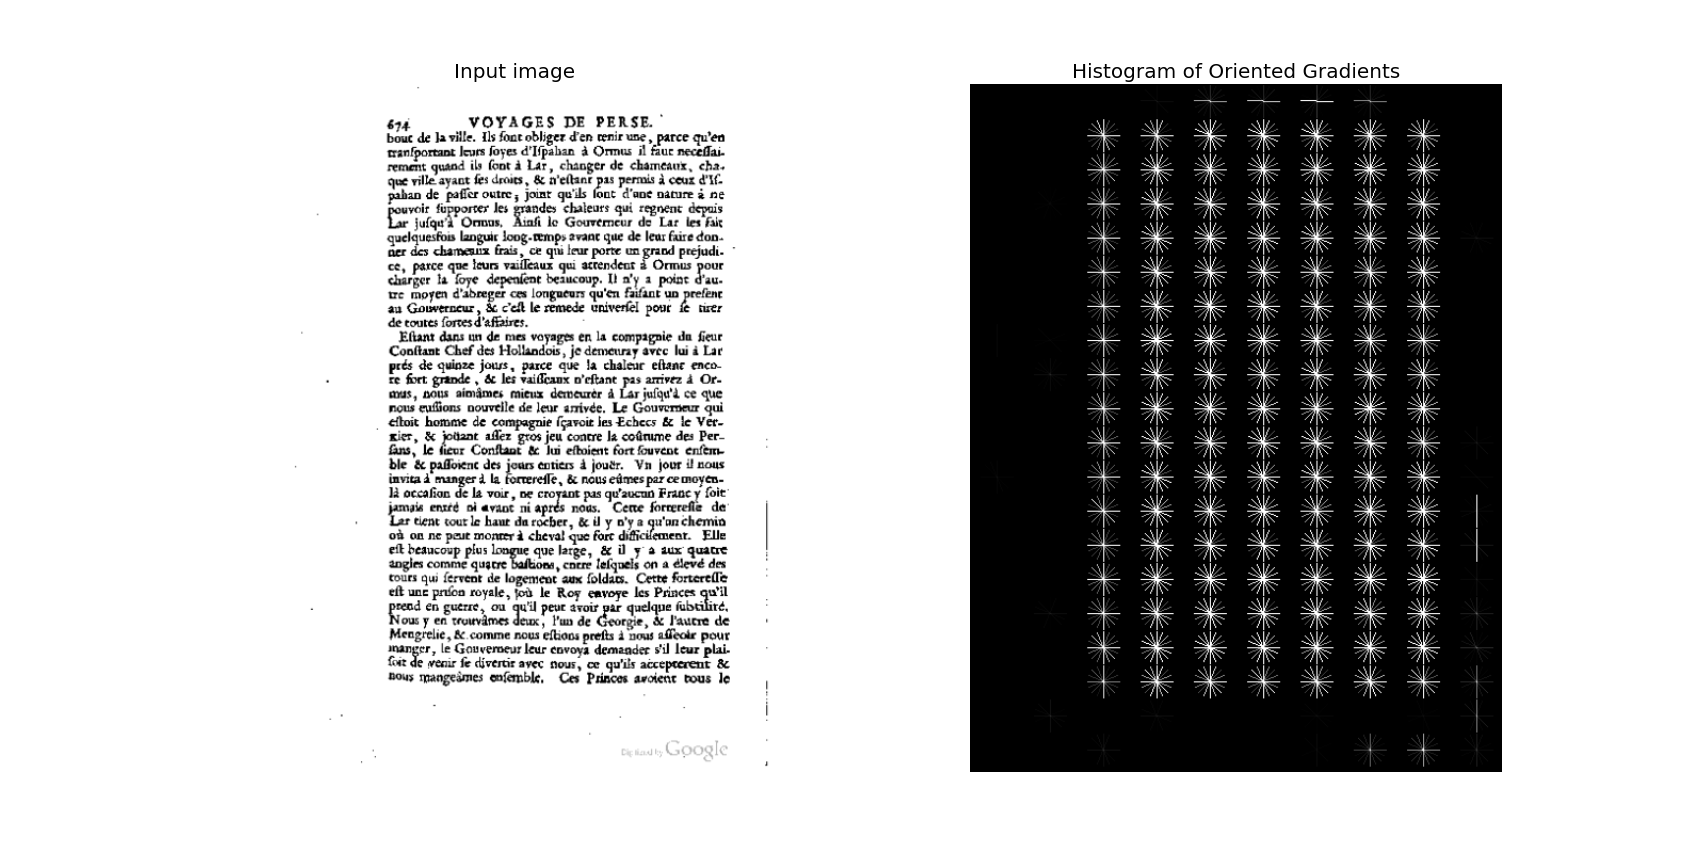
\includegraphics[trim=200px 0px 100px 0px, clip=true, width=.8\paperwidth]{resources/text1}\\
\framebreak
	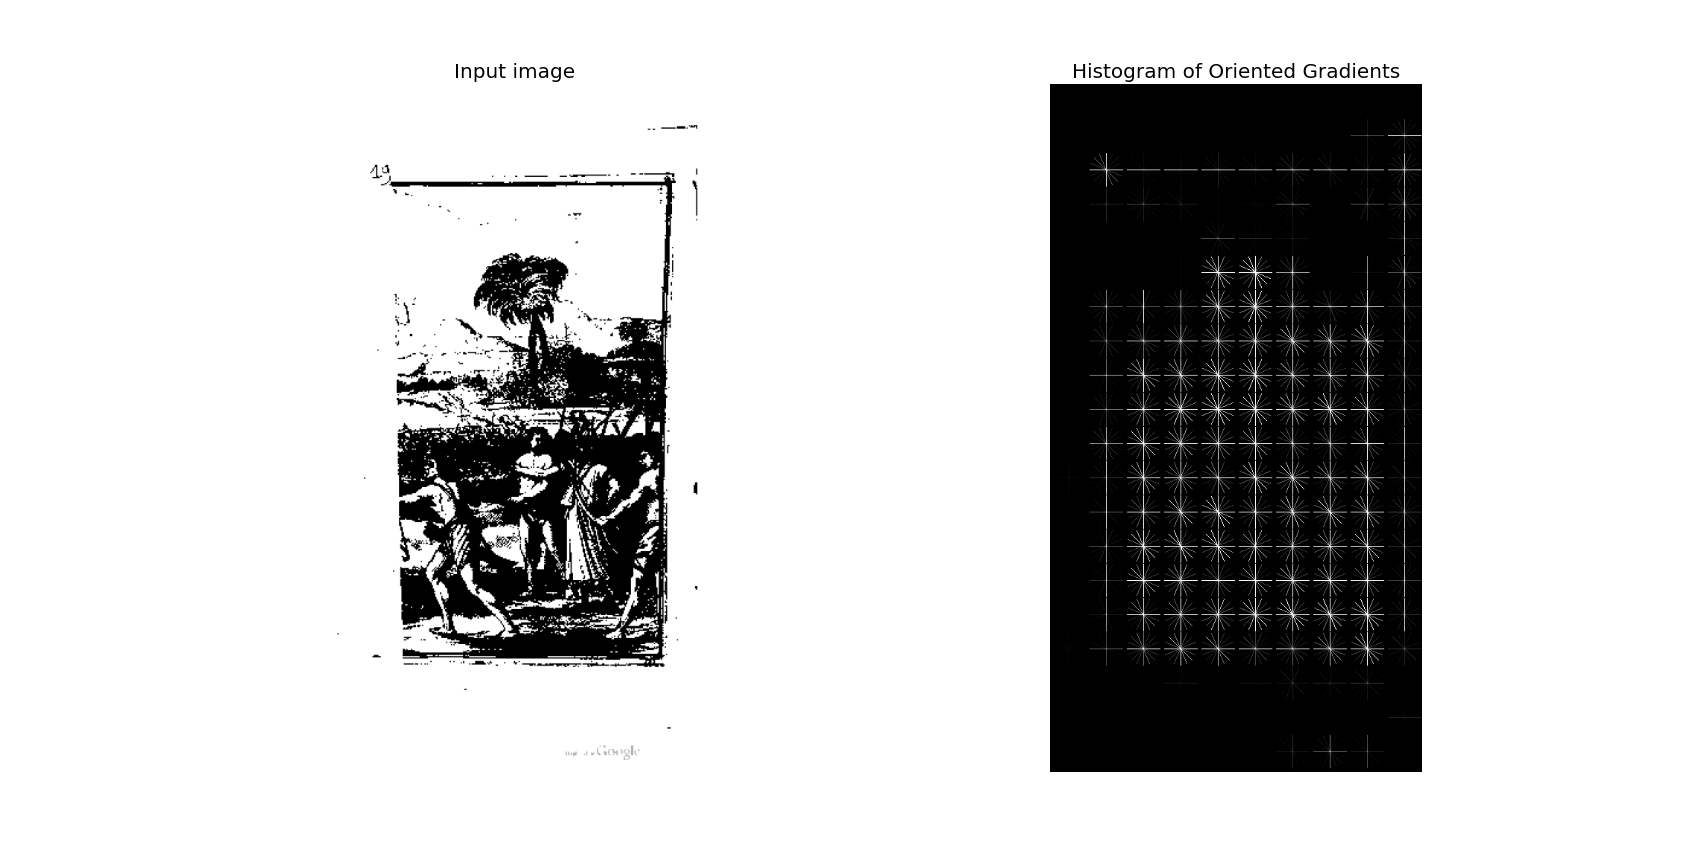
\includegraphics[trim=200px 0px 100px 0px, clip=true, width=.8\paperwidth]{resources/image1}\\
\framebreak
	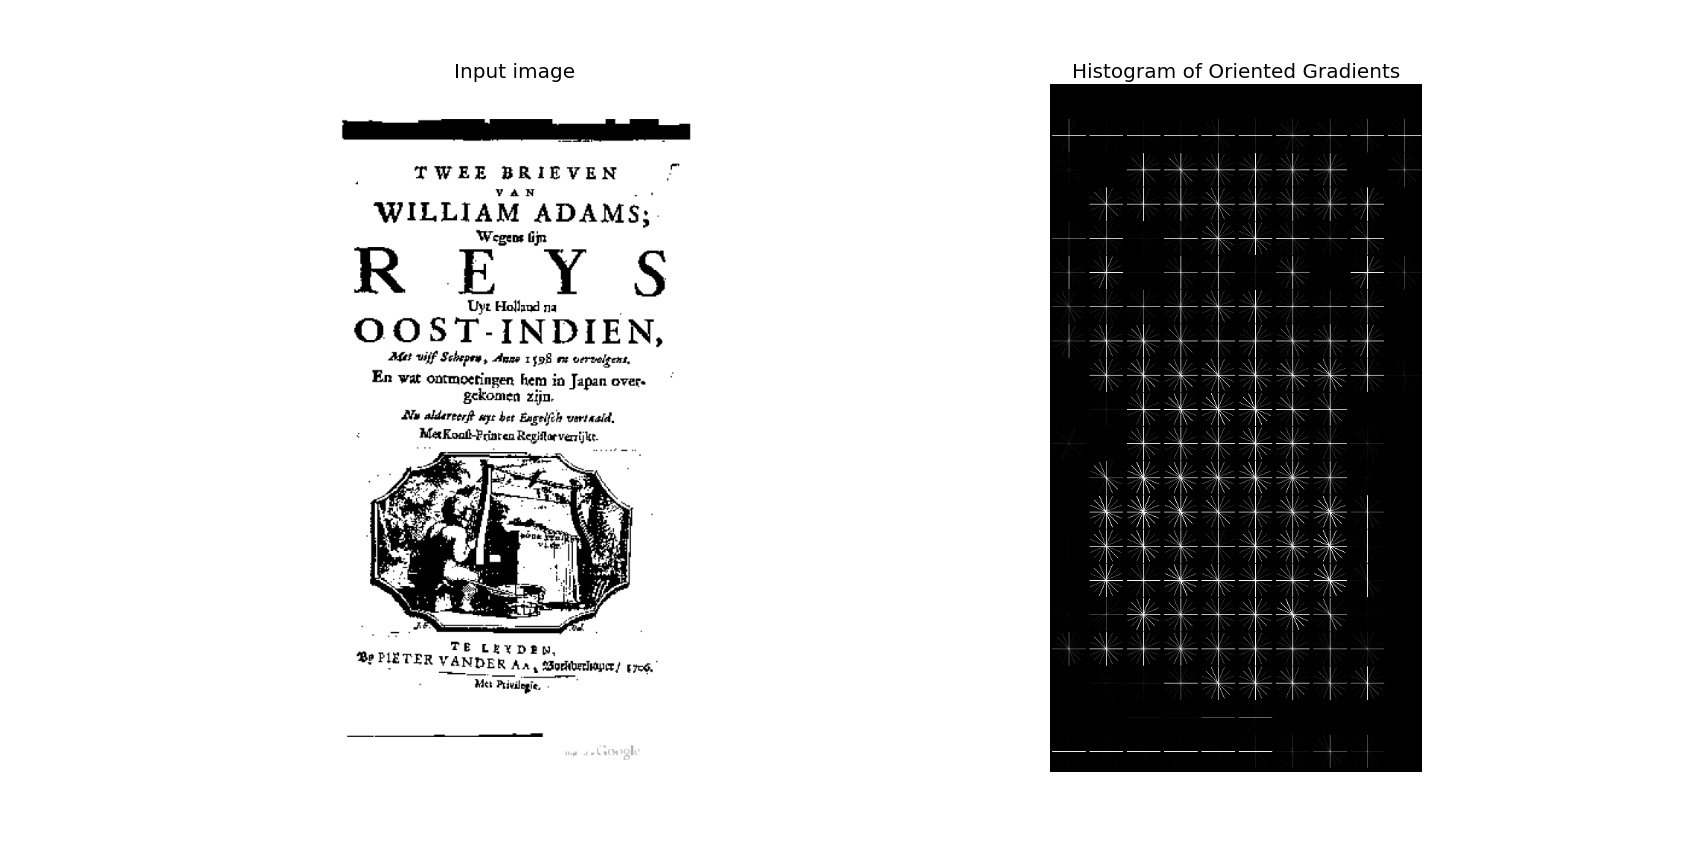
\includegraphics[trim=200px 0px 100px 0px, clip=true, width=.8\paperwidth]{resources/text_and_image1}
\end{frame}

% Explain SVM i.c.w. HOG features for pages
% Moved to introduction
% \slide{Classification using SVM}
% {
% 	\begin{itemize}
% 		\item All pages are annotated with having either ``text'', ``images'' or
% 		``nothing useful'' on it. Images get bounding boxes, which we will later
% 		use.
% 		\item Calculate 5x5 HOG features per page
% 		\item Train a Support Vector Machine (SVM) on these feature vectors and
% 		labels
% 		\item Predict whether a page contains an image based on this SVM
% 	\end{itemize}
% }

\begin{frame}
\frametitle{Test - Validation}
\begin{itemize}
\item Merge the sets of all annoated book pages into one set
\item Split this set into train set ($80\%$) and validation set($20\%$)
\item Use validation set to set parameters ($C$)
\end{itemize}


\end{frame}

\subsection{Results}
\begin{frame}
\frametitle{Results}
\begin{itemize}
\item Run the learned classifier on new books
\item Use F2-score in order to focus on recall (preprocess for annotator)
\end{itemize}
TODO: list results

\end{frame}
